\documentclass[12pt]{beamer}
 
\usetheme[white,sections]{Wisconsin}
\usepackage{fancyvrb}
\usepackage{color}
\usepackage[normalem]{ulem}
\usepackage{xcolor}
\usepackage{anyfontsize}
\usepackage{wrapfig}
\usepackage{graphicx}
\usepackage{verbatim}
\usepackage{framed}
\usepackage{listings}
\usepackage{showexpl}
\usepackage{xcolor}
\usepackage{lipsum}
\usepackage{hyperref}
\usepackage{subfigure}
\usepackage{animate,media9,movie15}

\lstset{%
basicstyle=\scriptsize\ttfamily, numbersep=2mm, numbers=left, numberstyle=\tiny, % number style
breaklines=true,frame=single,framexleftmargin=0mm, xleftmargin=3mm,
prebreak = \raisebox{0ex}[0ex][0ex]{\ensuremath{\hookleftarrow}},
backgroundcolor=\color{green!5},frameround=fttt,escapeinside=??,
rulecolor=\color{red},
morekeywords={% Give key words here                                         % keywords
    maketitle},
keywordstyle=\color[rgb]{0,0,1},                    % keywords
        commentstyle=\color[rgb]{0.133,0.545,0.133},    % comments
        stringstyle=\color[rgb]{0.627,0.126,0.941}  % strings
%columns=fullflexible 
}%

\lstdefinelanguage{myTeX}{
  language=TeX,
  morekeywords={begin, frac, end, ref, item, label, hline, cite, author, title, year, bibliographystyle, bibliography, column, documentclass, usetheme, @book, lstset},
  morecomment=[l]{\%},
  sensitive=true
}

\usepackage{tikz}
\usetikzlibrary{shapes.arrows}
\usetikzlibrary{positioning}
\usetikzlibrary{decorations.pathreplacing}
\tikzset{
    myarrow/.style={
        draw,
        fill=orange,
        single arrow,
        minimum height=4ex,
        single arrow head extend=1ex
    }
}
\tikzset{
    mydoublearrow/.style={
        draw,
        fill=orange,
        double arrow,
        minimum height=10.5ex,
        single arrow head extend=1ex
    }
}

\newcommand{\arrowup}{%
\tikz [baseline=-0.5ex]{\node [myarrow,rotate=90] {};}
}
\newcommand{\arrowdown}{%
\tikz [baseline=-1ex]{\node [myarrow,rotate=-90] {};}
}
\newcommand{\arrowright}{%
\tikz [baseline=-0.5ex]{\node [myarrow,rotate=0] {};}
}
\newcommand{\doublearrow}{%
\tikz [baseline=-1ex]{\node [mydoublearrow,rotate=0] {};}
}

\begin{document}
\newcommand*{\alphabet}{ABCDEFGHIJKLMNOPQRSTUVWXYZabcdefghijklmnopqrstuvwxyz}
\newlength{\highlightheight}
\newlength{\highlightdepth}
\newlength{\highlightmargin}
\setlength{\highlightmargin}{2pt}
\settoheight{\highlightheight}{\alphabet}
\settodepth{\highlightdepth}{\alphabet}
\addtolength{\highlightheight}{\highlightmargin}
\addtolength{\highlightdepth}{\highlightmargin}
\addtolength{\highlightheight}{\highlightdepth}
\setbeamertemplate{bibliography entry title}{}
\setbeamertemplate{bibliography entry location}{}
\setbeamertemplate{bibliography entry note}{}
\newcommand*{\Highlight}{\rlap{\textcolor{HighlightBackground}{\rule[-\highlightdepth]{\linewidth}{\highlightheight}}}}
\setbeamertemplate{bibliography item}[text]
\setbeamercolor{section in toc}{fg=white}
\setbeamercolor{bibliography entry author}{fg=black}
\setbeamercolor{bibliography item}{fg=black}
\setbeamercolor*{bibliography entry title}{fg=black}
%\setbeamerfont{section number projected}{size=\tiny}
\setbeamerfont{section number projected}{size=\fontsize{6}{6}\selectfont}
%\setbeamerfont{toc}{color=white}
\setbeamercolor{section number projected}{bg=UWRed,fg=white}
\hypersetup{linkcolor=white,urlcolor=white}

\AtBeginSection{\begin{frame}[plain] \sectionpage \end{frame}}

\defbeamertemplate{section page}{mine}[1][]{%
  \begin{centering}
    {\usebeamerfont{section name}\usebeamercolor[fg]{section name}#1}
    \vskip1em\par
    \begin{beamercolorbox}[sep=12pt,center]{part title}
      \usebeamerfont{section title}\insertsection\par
    \end{beamercolorbox}
  \end{centering}
\addtocounter{framenumber}{-1}
}

\setbeamertemplate{section page}[mine]


%TITLE PAGE
%%%%%%%%%%%%%%%%%%%%%%%%%%%%%%%%%%%%%%%%%%%%%%%%%%%%%%%%%%%%%%%%%%%%%%%%%%%%%%%%
\title{\LaTeX \, and Beamer}   
\author{Elliott Biondo}
\institute{University of Wisconsin - Madison}
\date{March 27, 2015}
\frame[plain]{\titlepage \addtocounter{framenumber}{-1}} 
%%%%%%%%%%%%%%%%%%%%%%%%%%%%%%%%%%%%%%%%%%%%%%%%%%%%%%%%%%%%%%%%%%%%%%%%%%%%%%%%
\section{Introduction}
%%%%%%%%%%%%%%%%%%%%%%%%%%%%%%%%%%%%%%%%%%%%%%%%%%%%%%%%%%%%%%%%%%%%%%%%%%%%%%%%
\begin{frame}{\LaTeX and Beamer}
\begin{itemize}
\item \LaTeX $\,$ is a markup language used to create documents.
\item Beamer is a \LaTeX $\,$ class used to make presentations.
\item Every aspect of this presentation was created in \LaTeX/Beamer.
\end{itemize}
\end{frame}

\begin{frame}{Why I use these tools}

\begin{itemize}
\item{Exacting control over every aspect of the document.}
\item{Powerful math mode.}
\item{Automatic bibliography tool (Bib\TeX).}
\item{Automatic handling of numbering and cross references to figures, tables, equations, citations.}
\item{Everything is text-based}
\begin{itemize}
\item{facilitates version control,}
\item{I can use my favorite editor.}
\end{itemize}
\end{itemize}
\end{frame}

\begin{frame}{Version Control}
When you use:
\begin{itemize}
\item \LaTeX/Beamer for typesetting,
\item MatPlotLib/GNUPlot for graphs,
\item GraphViz for flowcharts,
\item TikZ for fancy figures,
\end{itemize}

you can version control every aspect of a document.\\
\end{frame}

%%%%%%%%%%%%%%%%%%%%%%%%%%%%%%%%%%%%%%%%%%%%%%%%%%%%%%%%%%%%%%%%%%%%%%%%%%%%%%%%
\section{\LaTeX}
%%%%%%%%%%%%%%%%%%%%%%%%%%%%%%%%%%%%%%%%%%%%%%%%%%%%%%%%%%%%%%%%%%%%%%%%%%%%%%%%
\begin{frame}[fragile]
\frametitle{Hello World!}

\begin{columns}[c]
\column{0.5\textwidth}
\begin{block}{\centering hello\_world.tex}
\lstinputlisting[language=myTeX, frame=single]{examples/hello_world.tex}
\end{block}
\column{0.05\textwidth}
\arrowright
\column{0.45\textwidth}
\fbox{\includegraphics[width=0.9\textwidth]{examples/hello_world.pdf}}
\end{columns}
\end{frame}
%%%%%%%%%%%%%%%%%%%%%%%%%%%%%%%%%%%%%%%%%%%%%%%%%%%%%%%%%%%%%%%%%%%%%%%%%%%%%%%%
\begin{frame}[fragile]
\frametitle{Let's make the font a little bigger...}

\begin{columns}[c]
\column{0.5\textwidth}
\begin{block}{\centering hello\_world2.tex}
\lstinputlisting[language=myTeX, frame=single]{examples/hello_world2.tex}
\end{block}
\column{0.05\textwidth}
\arrowright
\column{0.45\textwidth}
\fbox{\includegraphics[width=0.9\textwidth]{examples/hello_world2.pdf}}
%\fbox{\includegraphics[trim={5cm 5cm 0cm 3cm},clip]{examples/hello_world2.pdf}}
\end{columns}
\end{frame}
%%%%%%%%%%%%%%%%%%%%%%%%%%%%%%%%%%%%%%%%%%%%%%%%%%%%%%%%%%%%%%%%%%%%%%%%%%%%%%%%
\begin{frame}[fragile]
\frametitle{Some Basics}

\begin{columns}[c]
\column{0.52\textwidth}
\begin{block}{\centering lists.tex}
\lstinputlisting[language=myTeX, frame=single, firstline=6, lastline=12, firstnumber=6]{examples/lists.tex}
\end{block}
\column{0.05\textwidth}
\arrowright
\column{0.44\textwidth}
\fbox{\includegraphics[width=0.9\textwidth]{examples/lists.pdf}}
\end{columns}
\end{frame}
%%%%%%%%%%%%%%%%%%%%%%%%%%%%%%%%%%%%%%%%%%%%%%%%%%%%%%%%%%%%%%%%%%%%%%%%%%%%%%%%
\begin{frame}[fragile]
\frametitle{Some Basics}

\begin{columns}[c]
\column{0.5\textwidth}
\begin{block}{\centering lists2.tex}
\lstinputlisting[language=myTeX, frame=single, firstline=6, lastline=16, firstnumber=6]{examples/lists2.tex}
\end{block}
\column{0.05\textwidth}
\arrowright
\column{0.45\textwidth}
\fbox{\includegraphics[width=0.9\textwidth]{examples/lists2.pdf}}
\end{columns}
\end{frame}
%%%%%%%%%%%%%%%%%%%%%%%%%%%%%%%%%%%%%%%%%%%%%%%%%%%%%%%%%%%%%%%%%%%%%%%%%%%%%%%%
\begin{frame}[fragile]
\frametitle{Math}

\begin{columns}[c]
\column{0.5\textwidth}
\begin{block}{\centering math.tex}
\lstinputlisting[language=myTeX, frame=single, firstline=6, lastline=13, firstnumber=6]{examples/math.tex}
Note that \texttt{\textbackslash label} works with equations, tables, figures, code listings, etc.
\end{block}
\column{0.05\textwidth}
\arrowright
\column{0.45\textwidth}
\fbox{\includegraphics[width=0.9\textwidth]{examples/math.pdf}}
\end{columns}
\end{frame}

%%%%%%%%%%%%%%%%%%%%%%%%%%%%%%%%%%%%%%%%%%%%%%%%%%%%%%%%%%%%%%%%%%%%%%%%%%%%%%%%
\begin{frame}[fragile]
\frametitle{Figures}

\begin{columns}[c]
\column{0.5\textwidth}
\begin{block}{\centering figure.tex}
\lstinputlisting[language=myTeX, frame=single, firstline=1, lastline=20, firstnumber=1]{examples/figure.tex}
\end{block}
\column{0.05\textwidth}
\arrowright
\column{0.45\textwidth}
\fbox{\includegraphics[width=0.9\textwidth]{examples/figure.pdf}}
\end{columns}
\end{frame}

%%%%%%%%%%%%%%%%%%%%%%%%%%%%%%%%%%%%%%%%%%%%%%%%%%%%%%%%%%%%%%%%%%%%%%%%%%%%%%%%
\begin{frame}[fragile]
\frametitle{Tables}

\begin{columns}[c]
\column{0.5\textwidth}
\begin{block}{\centering table.tex}
\lstinputlisting[language=myTeX, frame=single, firstline=7, lastline=14, firstnumber=7]{examples/table.tex}
\end{block}
\column{0.05\textwidth}
\arrowright
\column{0.45\textwidth}
\fbox{\includegraphics[width=0.9\textwidth]{examples/table.pdf}}
\end{columns}
\end{frame}
%%%%%%%%%%%%%%%%%%%%%%%%%%%%%%%%%%%%%%%%%%%%%%%%%%%%%%%%%%%%%%%%%%%%%%%%%%%%%%%%
\begin{frame}[fragile]
\frametitle{Code listings}

\begin{columns}[c]
\column{0.5\textwidth}
\begin{block}{\centering listings.tex}
\lstinputlisting[language=myTeX, frame=single, firstline=9, lastline=15, firstnumber=9]{examples/listing.tex}
(with \texttt{\textbackslash usepackage\{listings\}}  in the preamble)
\end{block}
\column{0.05\textwidth}
\arrowright
\column{0.45\textwidth}
\fbox{\includegraphics[width=0.9\textwidth]{examples/listing.pdf}}
\end{columns}
\end{frame}

%%%%%%%%%%%%%%%%%%%%%%%%%%%%%%%%%%%%%%%%%%%%%%%%%%%%%%%%%%%%%%%%%%%%%%%%%%%%%%%%
\begin{frame}[fragile]
\frametitle{References}

\begin{columns}[c]
\column{0.5\textwidth}
\begin{block}{\centering gravity.tex}
\lstinputlisting[language=mytex, frame=single, firstline=6, lastline=10, firstnumber=6]{examples/gravity.tex}
\end{block}
\begin{block}{\centering refs.bib}
\lstinputlisting[language=mytex, frame=single, firstline=1, lastline=7, firstnumber=1]{examples/refs.bib}
Note: need to run pdflatex {\bf and} bibtex.
\end{block}
\column{0.05\textwidth}
\arrowright
\column{0.45\textwidth}
\fbox{\includegraphics[width=0.9\textwidth]{examples/gravity.pdf}}
\end{columns}
\end{frame}

%%%%%%%%%%%%%%%%%%%%%%%%%%%%%%%%%%%%%%%%%%%%%%%%%%%%%%%%%%%%%%%%%%%%%%%%%%%%%%%%
\section{Beamer}
%%%%%%%%%%%%%%%%%%%%%%%%%%%%%%%%%%%%%%%%%%%%%%%%%%%%%%%%%%%%%%%%%%%%%%%%%%%%%%%%
\begin{frame}[fragile]
\frametitle{Beamer}

\begin{itemize}
\item Beamer is just a \LaTeX \, document class for making presentations.
\item Everything mentioned so far also applies to Beamer!
\end{itemize}

\end{frame}
%%%%%%%%%%%%%%%%%%%%%%%%%%%%%%%%%%%%%%%%%%%%%%%%%%%%%%%%%%%%%%%%%%%%%%%%%%%%%%%%
\begin{frame}[fragile]
\frametitle{Beamer Hello World!}

\begin{columns}[c]
\column{0.5\textwidth}
\begin{block}{\centering beamer\_hello.tex}
\lstinputlisting[language=myTeX, frame=single]{examples/beamer_hello.tex}
\end{block}
\column{0.05\textwidth}
\arrowright
\column{0.45\textwidth}
\fbox{\includegraphics[width=0.9\textwidth]{examples/beamer_hello.pdf}}
\end{columns}
\end{frame}
%%%%%%%%%%%%%%%%%%%%%%%%%%%%%%%%%%%%%%%%%%%%%%%%%%%%%%%%%%%%%%%%%%%%%%%%%%%%%%%%
\begin{frame}[fragile]
\frametitle{Columns}

\begin{columns}[c]
\column{0.5\textwidth}
\begin{block}{columns.tex}
\lstinputlisting[language=myTeX, frame=single, firstline=4, lastline=14, firstnumber=4]{examples/columns.tex}
\end{block}
\column{0.05\textwidth}
\arrowright
\column{0.45\textwidth}
\fbox{\includegraphics[width=0.9\textwidth]{examples/columns.pdf}}
\end{columns}
\end{frame}
%%%%%%%%%%%%%%%%%%%%%%%%%%%%%%%%%%%%%%%%%%%%%%%%%%%%%%%%%%%%%%%%%%%%%%%%%%%%%%%%
\begin{frame}[fragile]
\frametitle{Blocks}

\begin{columns}[c]
\column{0.5\textwidth}
\begin{block}{\centering blocks.tex:}
\lstinputlisting[language=myTeX, frame=single, firstline=5, lastline=21, firstnumber=5]{examples/blocks.tex}
\end{block}
\column{0.05\textwidth}
\arrowright
\column{0.45\textwidth}
\fbox{\includegraphics[width=0.9\textwidth]{examples/blocks.pdf}}
\vspace{0.5cm}
\end{columns}
\end{frame}
%%%%%%%%%%%%%%%%%%%%%%%%%%%%%%%%%%%%%%%%%%%%%%%%%%%%%%%%%%%%%%%%%%%%%%%%%%%%%%%%
\begin{frame}[plain]
\centerline{Okay, you get the the picture with the syntax.}
\end{frame}
%%%%%%%%%%%%%%%%%%%%%%%%%%%%%%%%%%%%%%%%%%%%%%%%%%%%%%%%%%%%%%%%%%%%%%%%%%%%%%%%
\section{More}
%%%%%%%%%%%%%%%%%%%%%%%%%%%%%%%%%%%%%%%%%%%%%%%%%%%%%%%%%%%%%%%%%%%%%%%%%%%%%%%%
\begin{frame}[fragile]
\frametitle{Pauses}

\begin{itemize}
\item{Spoon}
\pause
\item{Feed}
\pause
\item{Your}
\pause
\item{Audience}
\pause
\item Just add \texttt{\textbackslash pause}.
\pause
\begin{itemize}
\item plays nicely with most features in Beamer.
\pause
\item notice that page number has not incremented.
\end{itemize}
\end{itemize}

\end{frame}
%%%%%%%%%%%%%%%%%%%%%%%%%%%%%%%%%%%%%%%%%%%%%%%%%%%%%%%%%%%%%%%%%%%%%%%%%%%%%%%%
\begin{frame}[fragile]
\frametitle{Subfigures}

\begin{figure}[htb]
\subfigure[Sheep uno]{
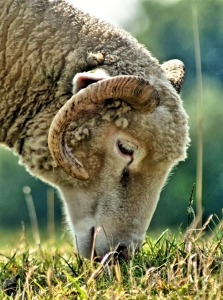
\includegraphics[width=2.3cm]{examples/sheep.jpg}
\label{subfig1}
}
\hspace{0.2cm}
\subfigure[Sheep dos]{
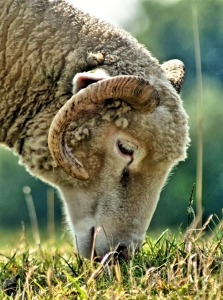
\includegraphics[width=2.3cm]{examples/sheep.jpg}
\label{subfig2}
}
\hspace{0.2cm}
\subfigure[Sheep tres]{
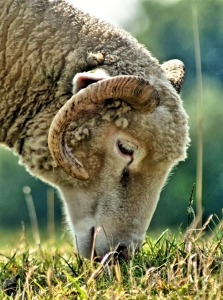
\includegraphics[width=2.3cm]{examples/sheep.jpg}
\label{subfig3}
}
\hspace{0.2cm}
\subfigure[\footnotesize Sheep quatro]{
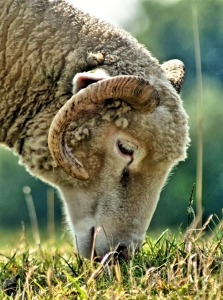
\includegraphics[width=2.3cm]{examples/sheep.jpg}
\label{subfig4}
}

\label{myfigure}
\caption{Caption of all sheep.}

Consider the sheep in Figure \ref{subfig2}...
\end{figure}
\end{frame}
%%%%%%%%%%%%%%%%%%%%%%%%%%%%%%%%%%%%%%%%%%%%%%%%%%%%%%%%%%%%%%%%%%%%%%%%%%%%%%%%
\begin{frame}[plain]
\frametitle{movie15 package}
\begin{figure}
\centering
  \includemovie[
    poster,
    autoplay,
    externalviewer,
    inline=false,
    text={\small(movie)}
  ]{6cm}{6cm}{pretty_movie.mp4}
\end{figure}
\end{frame}
%%%%%%%%%%%%%%%%%%%%%%%%%%%%%%%%%%%%%%%%%%%%%%%%%%%%%%%%%%%%%%%%%%%%%%%%%%%%%%%%
\begin{frame}[plain]
\frametitle{TikZ package}
\begin{itemize}
\item My new favorite thing
\item \href{http://www.texample.net/tikz/examples/3d-cone/}{3D Cone by Gene Ressler \color{blue}{[\uline{Link}]}}
\end{itemize}
% Author: Gene Ressler. Adapted to TikZ by Kjell Magne Fauske.
% See http://www.frontiernet.net/~eugene.ressler/ for more details
\begin{figure}
\centering
\begin{tikzpicture}[join=round]
    \tikzstyle{conefill} = [fill=blue!20,fill opacity=0.8]
    \tikzstyle{ann} = [fill=white,font=\footnotesize,inner sep=1pt]
    \tikzstyle{ghostfill} = [fill=white]
         \tikzstyle{ghostdraw} = [draw=black!50]
    \filldraw[conefill](-.775,1.922)--(-1.162,.283)--(-.274,.5)
                        --(-.183,2.067)--cycle;
    \filldraw[conefill](-.183,2.067)--(-.274,.5)--(.775,.424)
                        --(.516,2.016)--cycle;
    \filldraw[conefill](.516,2.016)--(.775,.424)--(1.369,.1)
                        --(.913,1.8)--cycle;
    \filldraw[conefill](-.913,1.667)--(-1.369,-.1)--(-1.162,.283)
                        --(-.775,1.922)--cycle;
    \draw(1.461,.107)--(1.734,.127);
    \draw[arrows=<->](1.643,1.853)--(1.643,.12);
    \filldraw[conefill](.913,1.8)--(1.369,.1)--(1.162,-.283)
                        --(.775,1.545)--cycle;
    \draw[arrows=->,line width=.4pt](.274,-.5)--(0,0)--(0,2.86);
    \draw[arrows=-,line width=.4pt](0,0)--(-1.369,-.1);
    \draw[arrows=->,line width=.4pt](-1.369,-.1)--(-2.1,-.153);
    \filldraw[conefill](-.516,1.45)--(-.775,-.424)--(-1.369,-.1)
                        --(-.913,1.667)--cycle;
    \draw(-1.369,.073)--(-1.369,2.76);
    \draw(1.004,1.807)--(1.734,1.86);
    \filldraw[conefill](.775,1.545)--(1.162,-.283)--(.274,-.5)
                        --(.183,1.4)--cycle;
    \draw[arrows=<->](0,2.34)--(-.913,2.273);
    \draw(-.913,1.84)--(-.913,2.447);
    \draw[arrows=<->](0,2.687)--(-1.369,2.587);
    \filldraw[conefill](.183,1.4)--(.274,-.5)--(-.775,-.424)
                        --(-.516,1.45)--cycle;
    \draw[arrows=<-,line width=.4pt](.42,-.767)--(.274,-.5);
    \node[ann] at (-.456,2.307) {$r_0$};
    \node[ann] at (-.685,2.637) {$r_1$};
    \node[ann] at (1.643,.987) {$h$};
    \path (.42,-.767) node[below] {$x$}
        (0,2.86) node[above] {$y$}
        (-2.1,-.153) node[left] {$z$};
    % Second version of the cone
    \begin{scope}[xshift=3.5cm]
    \filldraw[ghostdraw,ghostfill](-.775,1.922)--(-1.162,.283)--(-.274,.5)
                                   --(-.183,2.067)--cycle;
    \filldraw[ghostdraw,ghostfill](-.183,2.067)--(-.274,.5)--(.775,.424) 
                                   --(.516,2.016)--cycle;
    \filldraw[ghostdraw,ghostfill](.516,2.016)--(.775,.424)--(1.369,.1)
                                   --(.913,1.8)--cycle;
    \filldraw[ghostdraw,ghostfill](-.913,1.667)--(-1.369,-.1)--(-1.162,.283)
                                   --(-.775,1.922)--cycle;
    \filldraw[ghostdraw,ghostfill](.913,1.8)--(1.369,.1)--(1.162,-.283)
                                   --(.775,1.545)--cycle;
    \filldraw[ghostdraw,ghostfill](-.516,1.45)--(-.775,-.424)--(-1.369,-.1)
                                   --(-.913,1.667)--cycle;
    \filldraw[ghostdraw,ghostfill](.775,1.545)--(1.162,-.283)--(.274,-.5)
                                   --(.183,1.4)--cycle;
    \filldraw[fill=red,fill opacity=0.5](-.516,1.45)--(-.775,-.424)--(.274,-.5)
                                         --(.183,1.4)--cycle;
    \fill(-.775,-.424) circle (2pt);
    \fill(.274,-.5) circle (2pt);
    \fill(-.516,1.45) circle (2pt);
    \fill(.183,1.4) circle (2pt);
    \path[font=\footnotesize]
            (.913,1.8) node[right] {$i\hbox{$=$}0$}
            (1.369,.1) node[right] {$i\hbox{$=$}1$};
    \path[font=\footnotesize]
            (-.645,.513) node[left] {$j$}
            (.228,.45) node[right] {$j\hbox{$+$}1$};
    \draw (-.209,.482)+(-60:.25) [yscale=1.3,->] arc(-60:240:.25);
    \fill[black,font=\footnotesize]
                    (-.516,1.45) node [above] {$P_{00}$}
                    (-.775,-.424) node [below] {$P_{10}$}
                    (.183,1.4) node [above] {$P_{01}$}
                    (.274,-.5) node [below] {$P_{11}$};
    \end{scope}
\end{tikzpicture}
\end{figure}
\end{frame}

%%%%%%%%%%%%%%%%%%%%%%%%%%%%%%%%%%%%%%%%%%%%%%%%%%%%%%%%%%%%%%%%%%%%%%%%%%%%%%%%
\begin{frame}
\frametitle{TikZ works nicely with pauses:}

\begin{figure}
\centering
\begin{tikzpicture}[scale=1.2]
        \draw[thick] (0,0) -- (5,0) -- (5,5) -- (0,5) -- (0,0);
    \draw (2.5, 5.5) node {mesh volume element $k$};
    \draw [decorate,decoration={brace,amplitude=10pt, mirror}] (0.1,-0.1) -- (4.9, -0.1) node [midway,yshift=-0.6cm] {$l_{k}$};
    \pause
    \filldraw[fill=orange, opacity=0.2] (0,0) -- (2.5cm,0mm) arc (-50:50:2cm) arc (50:-41:-1.35cm) -- (2.36,5) --(0,5);
    \filldraw[fill=blue, opacity=0.2] (5,0) -- (2.5, 0) arc (-50:50:2cm) arc (50:-41:-1.35cm) -- (2.36,5) --(5,5);
    \draw[color=orange] (1,4) node {cell $a$};
    \draw[color=blue] (4,4) node {cell $b$};
    \pause
    \pause
    \draw[thick, ->, color=red] (0,1) -- (5,1) node[midway,above] {ray 1};
    \draw [decorate,decoration={brace,amplitude=10pt, mirror}, color=orange] (0.1,0.9) -- (3.05,0.9) node [orange,midway,yshift=-0.6cm] {$l_{1,a}$};
    \draw [decorate,decoration={brace,amplitude=10pt, mirror}, color=blue] (3.15,0.9) -- (4.9,0.9) node [blue,midway,yshift=-0.6cm] {$l_{1,b}$};
    \pause
    \draw[thick, ->, color=red] (0,3.5) -- (5,3.5) node[midway,above] {ray 2};
    \draw [decorate,decoration={brace,amplitude=10pt, mirror}, color=orange] (0.1,3.4) -- (2.15,3.4) node [orange,midway,yshift=-0.6cm] {$l_{2,a}$};
    \draw [decorate,decoration={brace,amplitude=10pt, mirror}, color=blue] (2.25,3.4) -- (4.9,3.4) node [blue,midway,yshift=-0.6cm] {$l_{2,b}$};
    \pause
    \draw[thick, ->, color=red] (0,2.5) -- (5,2.5) node[midway,above] {ray 3};
    \draw [decorate,decoration={brace,amplitude=10pt, mirror}, color=orange] (0.1,2.4) -- (2.95, 2.4) node [orange,midway,yshift=-0.6cm] {$l_{2,a}$};
    \draw [decorate,decoration={brace,amplitude=10pt, mirror}, color=blue] (3.05,2.4) -- (4.9,2.4) node [blue,midway,yshift=-0.6cm] {$l_{2,b}$};
    \onslide<1->
\end{tikzpicture}
\end{figure}

\end{frame}
%%%%%%%%%%%%%%%%%%%%%%%%%%%%%%%%%%%%%%%%%%%%%%%%%%%%%%%%%%%%%%%%%%%%%%%%%%%%%%%%
\begin{frame}{The downsides}

\begin{itemize}
\item Steep learning curve.
\begin{itemize}
\item You have to be willing to Google/StackOverflow things.
\item Until you are proficient, making documents takes much longer than using the alternatives.
\item You will occasionally have to ``hack'' things if you don't know how to do it the right way.
\end{itemize}
\item Commenting on .pdfs is inferior to the MS Word comments + accept/reject changes workflow.
\end{itemize}

\end{frame}

%%%%%%%%%%%%%%%%%%%%%%%%%%%%%%%%%%%%%%%%%%%%%%%%%%%%%%%%%%%%%%%%%%%%%%%%%%%%%%%%
\begin{frame}{Getting Started}

Latex:
\begin{itemize}
\item{Online tools}
\begin{itemize}
\item \href{https://www.overleaf.com/}{Overleaf \color{blue}{[\uline{Link}]}}
\item \href{https://www.sharelatex.com/}{ShareLaTeX \color{blue}{[\uline{Link}]}}
\end{itemize}

\item{GUI's}
\begin{itemize}
\item \href{http://www.lyx.org/}{LyX \color{blue}{[\uline{link}]}}
\item \href{http://www.xm1math.net/texmaker/}{Texmaker \color{blue}{[\uline{Link}]}}
\end{itemize}

\item{Command-line}
\begin{itemize}
\item \texttt{>> sudo apt-get install texlive-full}
\item \texttt{>> pdflatex mydoc.tex}
\end{itemize}

\end{itemize}
Beamer:
\begin{itemize}
\item \href{https://github.com/travitch/uw-beamer-template}{UW Beamer Template \color{blue}{[\uline{Link}]}}
\end{itemize}

\end{frame}
%%%%%%%%%%%%%%%%%%%%%%%%%%%%%%%%%%%%%%%%%%%%%%%%%%%%%%%%%%%%%%%%%%%%%%%%%%%%%%%%
\section*{Questions?}
%%%%%%%%%%%%%%%%%%%%%%%%%%%%%%%%%%%%%%%%%%%%%%%%%%%%%%%%%%%%%%%%%%%%%%%%%%%%%%%%
%%%%%%%%%%%%%%%%%%%%%%%%%%%%%%%%%%%%%%%%%%%%%%%%%%%%%%%%%%%%%%%%%%%%%%%%%%%%%%%%
%%%%%%%%%%%%%%%%%%%%%%%%%%%%%%%%%%%%%%%%%%%%%%%%%%%%%%%%%%%%%%%%%%%%%%%%%%%%%%%%
\end{document}
%%%%%%%%%%%%%%%%%%%%%%%%%%%%%%%%%%%%%%%%%%%%%%%%%%%%%%%%%%%%%%%%%%%%%%%%%%%%%%%%
%%%%%%%%%%%%%%%%%%%%%%%%%%%%%%%%%%%%%%%%%%%%%%%%%%%%%%%%%%%%%%%%%%%%%%%%%%%%%%%%
